\documentclass{article}
\usepackage{graphicx}
\usepackage{mathtools}
\DeclarePairedDelimiter\floor{\lfloor}{\rfloor}

\begin{document}
\section{Discrete Cmac}
\subsection{Description}
 \begin{enumerate}
   \item \textbf{Define input space} - In the implementation, the input space was defined over the range[0,10]
   \item \textbf{Association Cells} - This is a 1D cmac, so the number of association cells was chosen to match the number
    weights.In the implementation,35 weights with 35 association cells.
   \item \textbf{Quantize input} - The input space is quantized so as to perform a table lookup. The quantization is achieved
     using the formula given below.
     \begin{equation}
       q_x = \floor*{resolution*\frac{x - xmax}{xmin-xmax}}
     \end{equation}
     so in the implementation, we have,
     \begin{equation}
       q_x = \floor*{35*\frac{x- 0}{10 - 0}}
     \end{equation}
   \item \textbf{Generalization Number, g} - This number indicates the degree of similarity between tasks. Odd numbers was utilized as centering weights around quantized input was preferable. When an input is received, the association cells activated are centered around the quantized input. For example, suppose the quantized input of 3 is 3 with a generalization number of 5, this means that 2 cells before 3(0 and 1) and 2 cells after 3(4 and 5) are activated.

 \end{enumerate}
\subsection{Results}
  \paragraph{Generalization Vs Convergence:}
   Clearly from the graph shown below,it can be noted that  
  as the generalization number increases, the model has a hard time converging.This can
  be attributed to the fact that the generalization number,g indicates to a degree the similarity
  between tasks. As g increases, the model becomes weak(wrong model) as it tends to consistently learn the wrong thing by categorizing unrelated tasks 
  as similar,hence a high bias. Ideally, g is chosen so that tasks which are related have similar values whiles tasks
  which are different have clear cut distinct values. 
  \begin{figure}[h!]
     \centering
    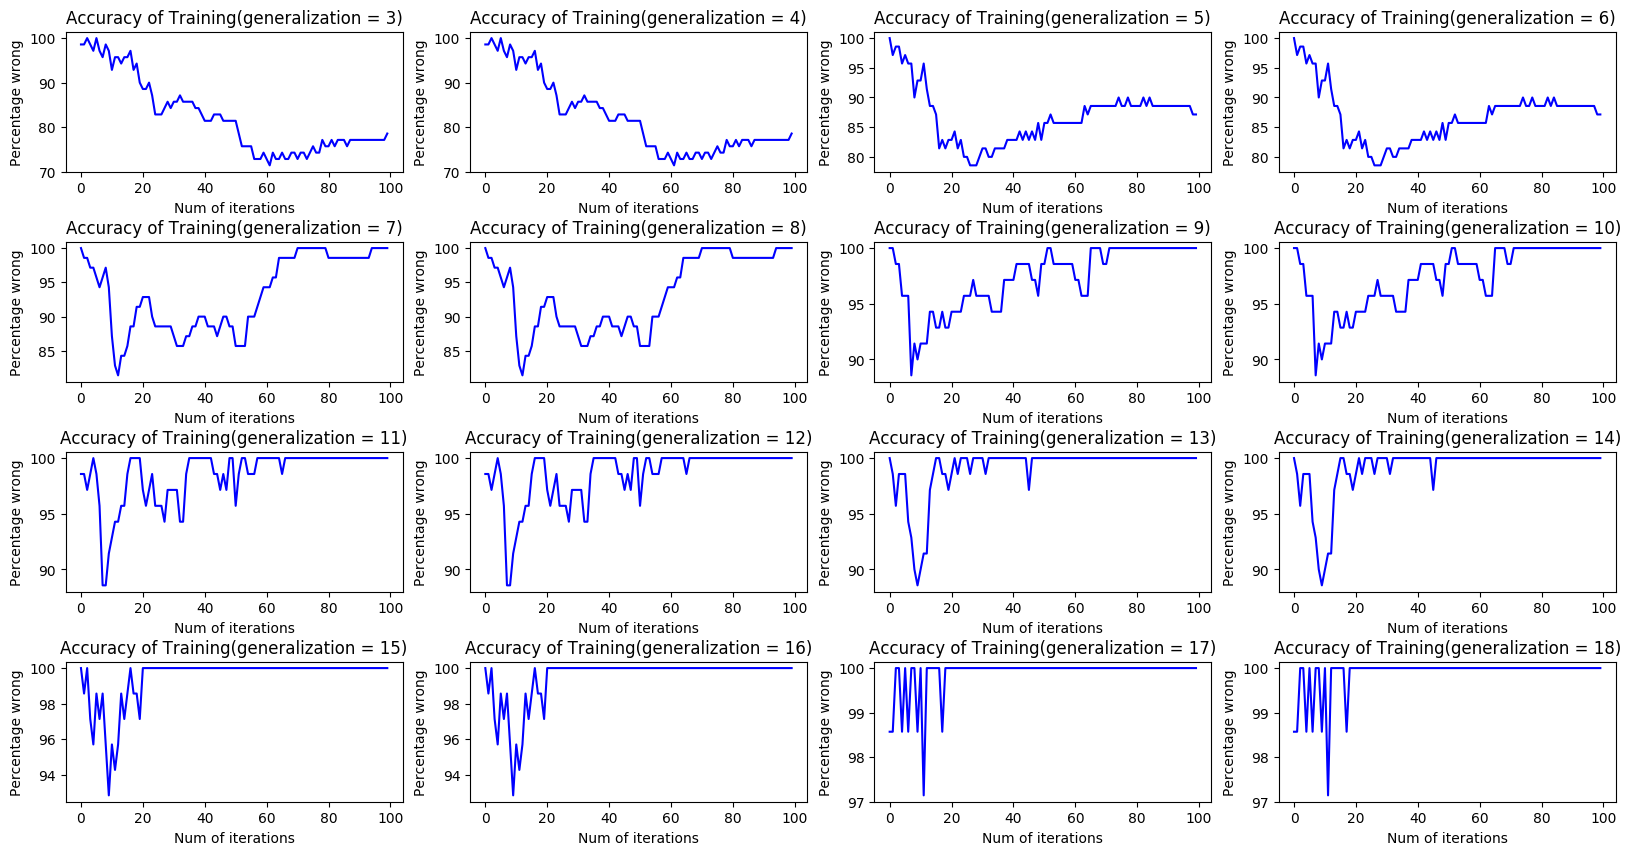
\includegraphics[scale=0.35]{./Results/convergenceVsgeneralization.png}
  \end{figure}

  \paragraph{Accuracy:}
    Below is a graph that depicts the accuracy of the Discrete Cmac. After running a couple of times, it can 
    be noted that the accuracy hovers between 70-85\%
  \begin{figure}[h!]
    \centering
    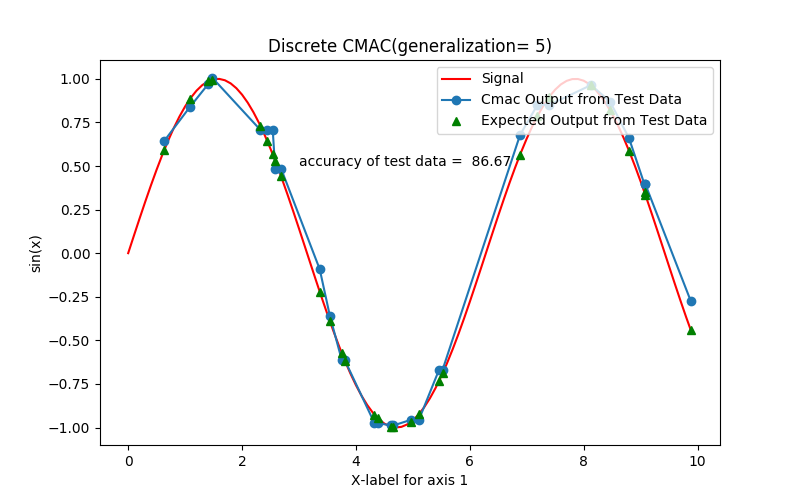
\includegraphics[scale=0.7]{./Results/discreteAccuracy.png}
  \end{figure}
\newpage 
\section{Continous Cmac}
%\subsection{Description}
\subsection{Results}
  \paragraph{Accuracy:}
    Below is a graph that depicts the accuracy of the Continous Cmac. After running the the code a couple of times, it can
    be noted that the accuracy hovers between 40-60\%
  \begin{figure}[h!]
     \centering
     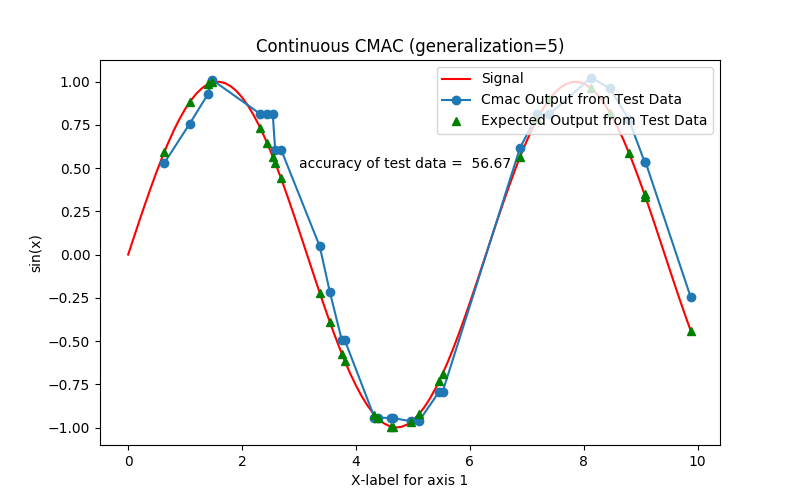
\includegraphics[scale=0.65]{./Results/continousAccuracy.png}
  \end{figure}
  \paragraph{Discrete Vs Continous Cmac:}
  The "convergence Vs generalization" graphs for both continous cmac and discrete cmac are relatively similar in particular for generalization numbers g = 3 to 6. However,the accuracy of the test results  are clearly different.
  For the same parameters used in training the Discrete Cmac(generalization number, number of iterations in training,accuracy used in training,learning rate), it can be noted that the continous Cmac has a significant drop in accuracy as the model clearly seems to overfit.This is because the continous cmac slides over more weights. Therefore, although a generalization number of 5 is used, more than 5 weights are changed during each update and this means that more inputs are categorized as similar and that is undesirable. To rectify this the generalization number can be reduced and number of iterations increased to improve perfomance. Also, the type of sliding window utilized has an impact on the results.  
  \begin{figure}[h!]
    \centering
    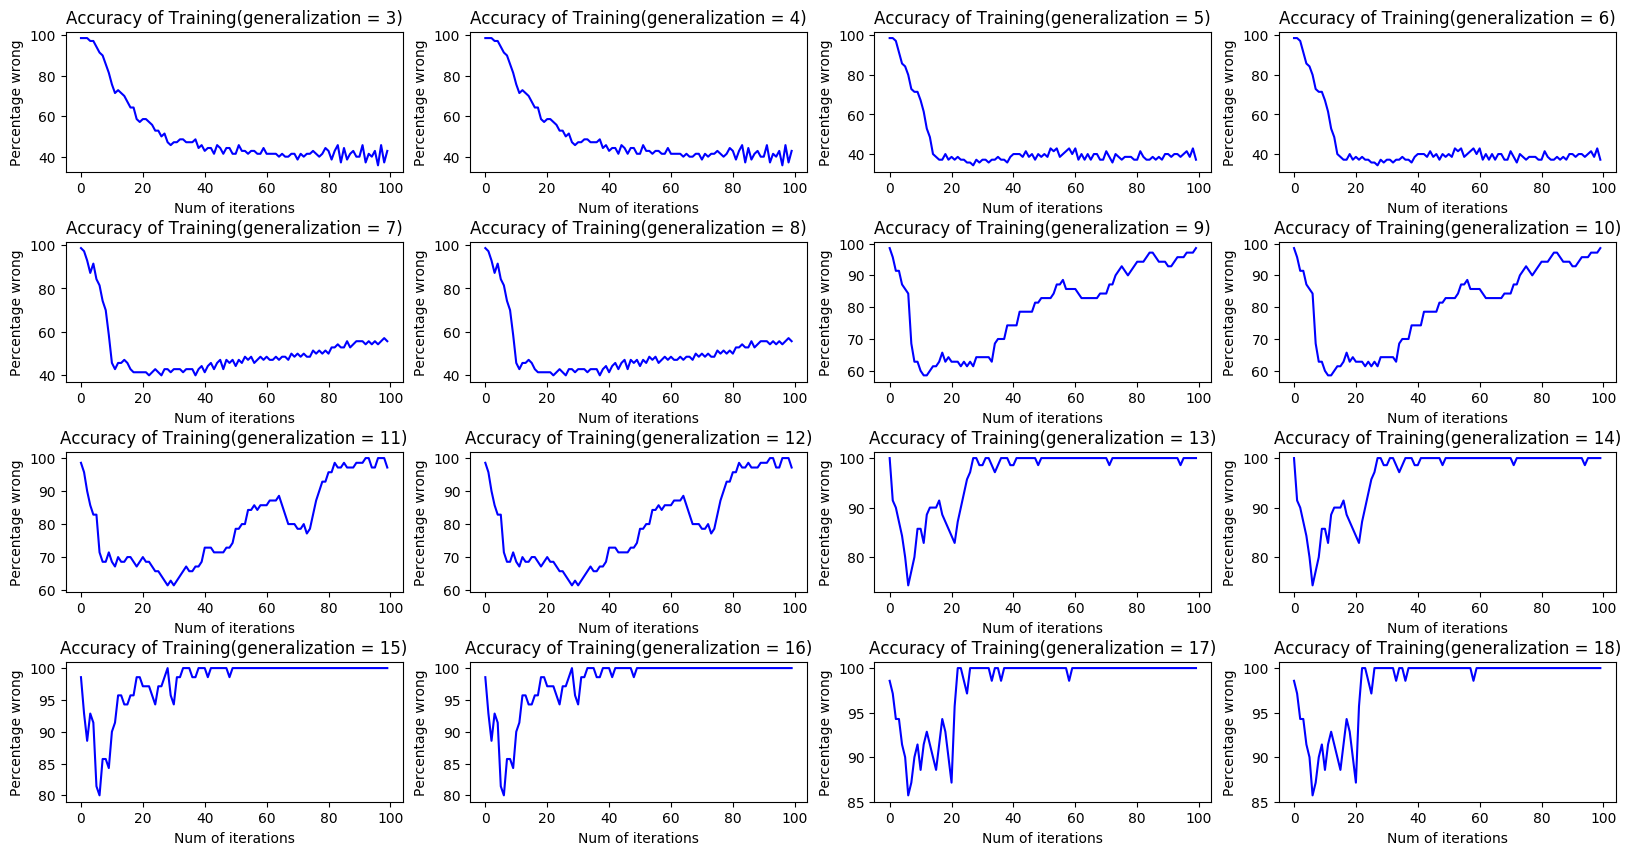
\includegraphics[scale=0.35]{./Results/convergenceVsgeneralizationC.png}
  \end{figure}
\newpage
\section{Recurrent Connections with Cmac}
\paragraph{Problem:}
Cmac can be particular useful in modelling connnections that are only state dependent. Most recurrent connections such as
recurrent neural networks employed in speech recognition, music generation etc. are temporally dependent. So if a given task
is paused midway, all the relevant information is lost as the history of the information seen previously matters.
Although changes can be made to such networks by storing certain information, this is usally intractable as it means a different logic to determine where the current function is located at. 
Therefore, a model that is only state dependent becomes necessary. Cmac can be used to model a state dependent recurrent connections and this is shown below. 

\paragraph{Modelling Cmac to output desired trajectory:}
The output of cmac is now fed as an input to P(logic depends on the particular problem), then P decodes
the appropriate weights to excite. This is illustrated by the diagram below.

  \begin{figure}[h!]
    \centering
    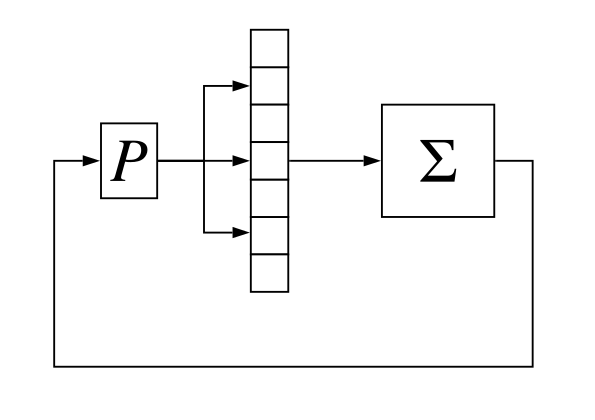
\includegraphics[scale=0.2]{./Data/statemodelling.png}
    \caption{Recurrent Cmac}
  \end{figure}

  \textbf{What if two different inputs have the same ouput value. How do we know which input to excite next?}
  \begin{figure}[h!]
    \centering
    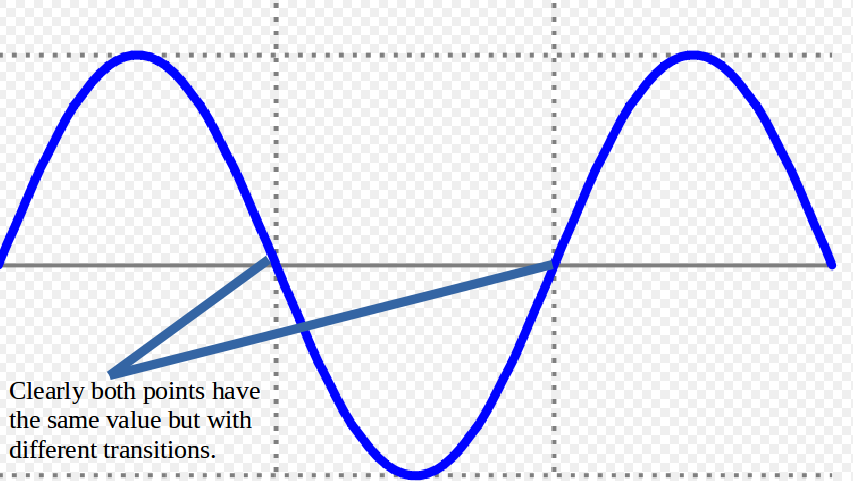
\includegraphics[scale=0.2]{./Data/model2.png}
    \caption{Trajectory}
  \end{figure} \\
  The decoding function \textbf{P} must take this into account. Therefore,  P is modified to be $P(\sum,weights)$. Therefore,
  different inputs with same output weight sum are treated as different. The diagram is now modified to be the following.

  \begin{figure}[h!]
    \centering
    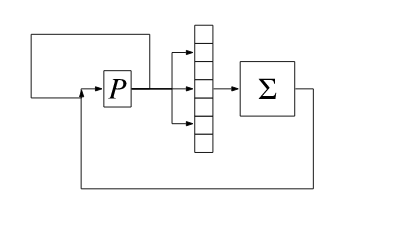
\includegraphics[scale=0.5]{./Data/modifiedmodel.png}
    \caption{Modified model}
  \end{figure} 
\end{document}


